\begin{frame}{Generalization: Data Augmentation}
    \framesubtitle{The Best Regularizer: More Data}
    \begin{itemize}
        \item One of the most effective ways to improve a model's generalization is simply to train it on more data.
        \item However, collecting and labeling new data can be expensive and time-consuming.
        \item \bhighlight{Data Augmentation} is a powerful technique to artificially expand the training dataset by creating modified, yet realistic, copies of existing data.
    \end{itemize}
\end{frame}

\begin{frame}{Data Augmentation}
    \framesubtitle{The Core Idea}
    \begin{itemize}
        \item The core idea is to apply transformations to an input example in a way that \bhighlight{does not change its label}.
        \item For example, a horizontally flipped image of a cat is still an image of a cat.
        \item This teaches the model to become \bhighlight{invariant} to these transformations, helping it focus on the true underlying features of the class rather than irrelevant variations in the input.
    \end{itemize}
\end{frame}

\begin{frame}{Data Augmentation}
    \framesubtitle{Examples for Image Data}
    \begin{figure}
        \centering
        % Source: Regularization.pdf, Page: 49
        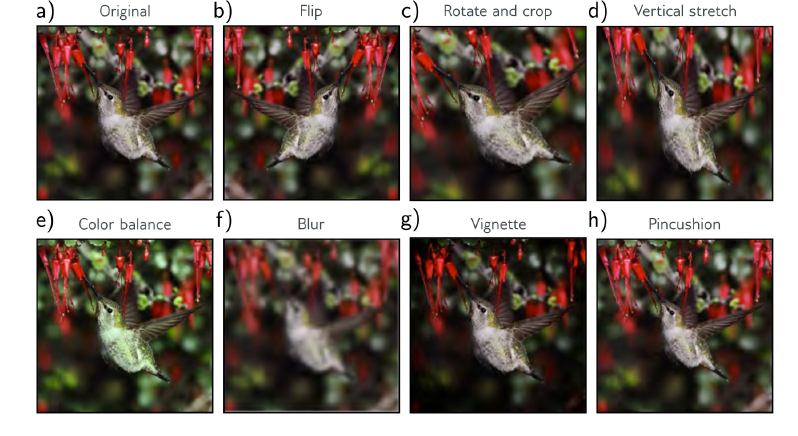
\includegraphics[width=\linewidth]{images/data_augmentation_examples.png}
        \caption{Common augmentation techniques for images include flipping, rotating, cropping, color shifting, blurring, and adding distortions.}
    \end{figure}
\end{frame}

\begin{frame}{Data Augmentation}
    \framesubtitle{Another Technique: Adding Noise}
    \begin{itemize}
        \item Another form of data augmentation is to add random noise directly to the input data.
        \item This can make the model more robust and less sensitive to small variations in the input, effectively acting as a regularizer.
    \end{itemize}
    \begin{figure}
        \centering
        % Source: Regularization.pdf, Page: 51
        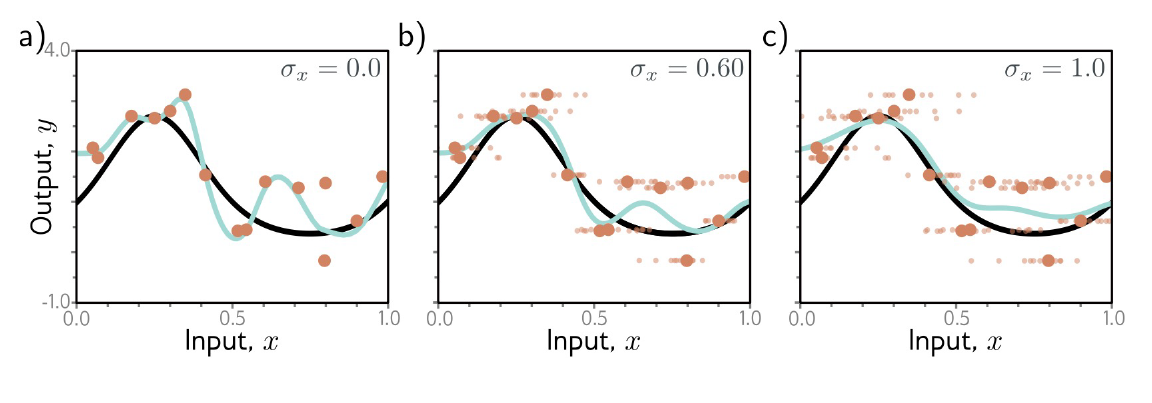
\includegraphics[width=0.8\linewidth]{images/augmentation_noise.png}
        \caption{The effect of adding increasing levels of noise ($\sigma_x$) to the input data during training.}
    \end{figure}
\end{frame}